
% XeLaTeX can use any Mac OS X font. See the setromanfont command below.
% Input to XeLaTeX is full Unicode, so Unicode characters can be typed directly into the source.

% The next lines tell TeXShop to typeset with xelatex, and to open and save the source with Unicode encoding.

%!TEX TS-program = xelatex
%!TEX encoding = UTF-8 Unicode

\documentclass[11pt]{article}


%%%%%%%%%%%%%%%
\def\Type{ApplicationDJ}
\def\TypeNum{The Keeling Curve and Climate Change}
\def\TypeTitle{Modeling Atmospheric CO$_2$\\
Key}
\def\Semester{Fall 2024}
\def\Course{Math 1190/1210}
%\def\Targets{{\bf\color{Goldenrod}AD1}}
\def\desmosClassCode{{\bf ZAJ$3$AZ}}

\usepackage{preambleDJ}

\captionsetup{font=small}

\begin{document}
\pagestyle{otherpages}
\thispagestyle{firstpage}
\vs{.8}
{\bf Introduction}\\

In our pre-class work, we introduced the Keeling Curve, which illustrates the dramatic rise in the concentration of carbon dioxide in the earth's atmosphere over the past half-century. We  attempted to model this curve with a linear function drawn through two points on the curve. In this application we will use the method of linear regression and other functions  to find the ``best fit'' line for the data, i.e., the  function that (in a precisely defined way) that matches the data as well as possible. We will use these new approaches to better predict  understand  the future concentration of CO$_2$ in our atmosphere and whether or not we are close to a `tipping point."

\vspace{0.5cm}


{\bf The Keeling Curve, Revisited}\\


Recall the following figure from the pre-class activity.\footnote{Monthly average CO2 concentrations (ppm) derived from flask air samples,  Mauna Loa, Hawaii. Source: R. F. Keeling and S. J. Walker, Scripps CO2 Program ( http://scrippsco2.ucsd.edu,ripps Institution of Oceanography (SIO) } 
\footnote{ C. D. Keeling, S. C. Piper, R. B. Bacastow, M. Wahlen, T. P. Whorf, M. Heimann, and   H. A. Meijer, Exchanges of atmospheric CO2 and 13CO2 with the terrestrial biosphere and   oceans from 1978 to 2000.  I. Global aspects, SIO Reference Series, No. 01-06, Scripps   Institution of Oceanography, San Diego, 88 pages, 2001. }\\
\graphicsC{keelingCurve.pdf}{5}{{\bf Figure 1:} The Keeling Curve}



\vspace{0.2cm}

As in the pre-class work, we are only considering the baseline concentration of CO$_2$ in parts per million (ppm), which is represented by the thick curve in Figure 1.  Baseline atmospheric CO$_2$ levels at five-year intervals from 1965 through 2010 are
\begin{center}
\begin{tabular}{|c|c|c|c|c|c|c|c|c|c|c|}
\hline
year & 1965 & 1970 & 1975 & 1980 & 1985 & 1990 & 1995 & 2000 & 2005 & 2010 \\
\hline
CO$_2$ level & 320 & 325 & 331 & 338 & 345 & 354 & 360 & 369 & 379 & 389 \\
\hline
\end{tabular}
\end{center}

This data can be found at \href{https://student.amplify.com/}{\underline{student.amplify.com}} or \href{https://student.desmos.com/}{\underline{student.desmos.com}} using code \desmosClassCode.  Look for ``During-Class: The Keeling Curve" in the To Do or Past Work Tab. You will also likely want to use this Desmos/Ampify activity to help answer the following questions.  
\newpage
\enum{
\item Use Desmos to find the line of best fit to this data.     See {\em Creating Functions and Functions of Best Fit in Desmos} at the end of this document for instructions on how to find this equation and $R^2$ value.
\tasksA{2}{
\task What is the equation of the line of best fit? Express your answer in slope-intercept form and round coefficients to four decimal places.\\
\blue{
This question was asked as part of the pre-class assignment.  Instructions to create the trendline are found on last page of the both the pre-class and during-class assignments.. Here's one way to create a linear trendline.  $$c_1\sim mt_1+b$$
}
\sol{
$$c(t)=1.5321\,t+316.527$$
}
\task What is the $R^2$ value rounded to $4$ decimal places? \\\\ 
\sol{
$$R^2=0.9913$$
}
}\vs{.5}
\item Why might someone want to use linear regression (i.e. line of best fit)  to model the Keeling Curve? Why not just ``eyeball'' (i.e. ``guess") a line of best fit?  \\
\sol{
There are several reasonable answers to this question. Here are two.
\itemI{
\item The most important reason to have a well-defined, agreed-upon, notion of "best fit" is that doing so allows scientists (or statisticians, etc.) to verify each other's results. Two different people looking at the same data may eyeball different lines, but using linear regression both will come up with the exact same lie of best fit. (Note that there are in fact other ways to define a "best fit" line mathematically, so one still needs to be careful! The advantage of linear regression over some other methods is that it is relatively easy to compute.) 
\item Another reason for having an agreed-upon method, defined with a specific mathematical formula, is that it may lead us to define other useful quantities, such as $R^2$.
}
}
%\item  How does the slope of the line of best fit compare to the slopes you found in the two linear functions calculated the pre-class ``Keeling Curve" activity? Which of these three functions do you think will do the best job predicting the actual CO$_2$ level in 2024? Why?  DO WE NEED TO PREDICT 2024 HERE?

\newpage
\item Now  experiment in Desmos with quadratic, exponential and logarithmic functions  to fit this same data set. See {\em Creating Functions and Functions of Best Fit in Desmos} at the end of this document for directions to create these in Desmos. Please round all coefficients and $R^2$ values to four decimal places. \label{qNum}\\
\blue{
See instructions at end of document to create trendlines (i.e. functions of best fit). 
}
\begin{enumerate}
\item \begin{tabular}{p{4in} l} What's the best-fitting quadratic function? & What is the $R^2$ value?\end{tabular}
\sol{
~\\
$\ds c_{quadratic}(t)=.0109\,t^2+1.0412\,t+319.8$\hfill$\ds R^2=0.9993$
}
\vs{.25}
\item \begin{tabular}{p{4in} l} What's the best-fitting exponential function? & What is the $R^2$ value?\end{tabular}
\sol{
~\\
$\ds c_{exponential}(t)=76.8748e^{0.0143 \, t}+242.763$\hfill$\ds R^2=0.9994$
}
\vs{.25}
\item\begin{tabular}{p{4in} l} What's the best-fitting logarithmic function? & What is the $R^2$ value?\end{tabular}
\sol{
~\\
$\ds c_{log}(t)=-109.128\ln\left( -0.0006t +0.0535\right)$\hfill$\ds R^2=0.9993$
}
\vs{.25}
\end{enumerate} 
 \item Some scientists believe that not only is the amount of CO$_2$ in the atmosphere growing, but that the growth rate is speeding up.  Which of the following best fit functions reflect this belief? Explain your thinking.
 \tasksA{3}{
 \task Linear best fit function
 \task Exponential best fit function.
 \task Logarithmic best fit function.  
 }
 \sol{

 \mpageT{.7}{.3}[\hs{.2}]{
 \itemI{
 \item Tangent lines of Linear functions {\em are} the linear function itself.  This means that tangent lines for all $t$ have the same slope.  Another way to say this is that linear functions have a constant Rate of Change.  This means that the linear function we found   {\em does not} reflect this belief.
 \item The exponential function we found gets steeper and steeper.  That is, the slope of tangent lines get steeper and steeper as $t$ gets larger and larger.  So our exponential function  {\em does} reflect this belief.
 }
 }{
 \begin{flushright}
     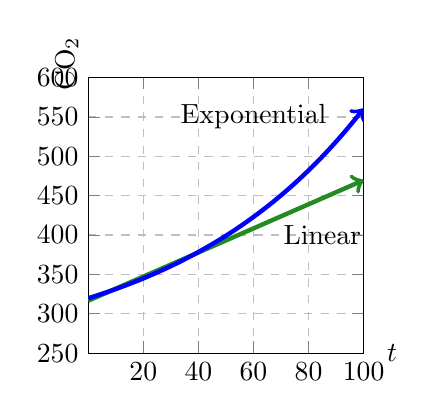
\begin{tikzpicture}[scale=1]
          \begin{axis}[
        %    axis y line = left,
        %    axis x line = bottom,
        	    ylabel={CO$_2$},
            xlabel={$t$},
            x label style={  at={(ticklabel* cs:1.05)},  anchor=west,},
            xtick       = {20,40,60,80,100},
            xticklabels = {$20$,$40$,$60$,$80$,$100$},
            ytick       = {250,300,350,400,450,500,550,600},
            yticklabels = {$250$,$300$,$350$,$400$,$450$,$500$,$550$,$600$},
            y label style={  at={(ticklabel* cs:1.05)},  anchor=south,},
            samples     = 160,
            domain      = 0:100,
            restrict y to domain=250:600,
            xmin = 0, xmax = 100,
            ymin = 250, ymax = 600,
            grid=both, grid style=dashed,
            width=2in, height=2in
          ]
          % pieces 1 and 2
          \addplot[domain=0:100, ForestGreen, ultra thick, ->] {1.5321*x+316.527};
           \node at (85,400) {\fgreen{Linear}};
           \addplot[domain=0:100, blue, ultra thick, ->] {76.8748*e^(.0142*x)+242.763};
             \node at (60,550) {Exponential};
         % \addplot[domain=0:100, red, ultra thick, ->] {-109.128*ln(-.0006*x+.0535)};
           % \draw[ultra thick, red, dashed, -] (89.17,250) -- (89.17,600);
           % \addplot[domain=0:60, blue, ultra thick, ->] {1.5 *x +316};
         % \node at (1,4) {$e^t$};
        \end{axis}
    \end{tikzpicture}
\captionof*{figure}{\blue{Graphs of linear and exponential trend lines.}}
    \end{flushright}
    }
\vs{-.3}\\
\itemI{
 \item The logarithmic function that we found also gets steeper and steeper. That is, the slope of tangent lines get steeper and steeper as $t$ gets larger and larger.  So our logarithmic function  {\em does} reflect this belief.
 \item But there is more going on here than might be clear at first. A typical trendline of the form $f(t)=\ln( t)$ grows at a slower and slower rate (see graph on left below). Additionally  $\ds 
 \lim_{t\to 0^+}\ln(t) =-\infty$ which means there is a vertical asymptote at $x=0$ (see graph on left below).
\item But, the trendline representing our logarithmic  model is is $$ c_{log}(t)=-109.128\ln\left( -0.0006t +0.0535\right)$$
The presence of  $ -0.0006t +0.0535$ inside the log function changes the location of the vertical asymptote.  In particular, when  $-0.0006t +0.0535=0$ , we will have a vertical asymptote. This occurs at $\ds t=\frac{535}{6}\approx 89.17$  (see graph in the middle below).
\item  Any logarithmic function is not defined at $0$ nor for negative values. Whenever $\ds t>\frac{535}{6}\approx 89.17$, $-0.0006t +0.0535<0$ and  {\em our logarithmic trend line is undefined.} Past $t\approx 89.17$, our logarithmic model is useless while both the exponential model and linear model keep predicting future values (see gray region on below right graph).
 }

\mpageTth{.35}{.35}{.35}{
  \begin{center}
     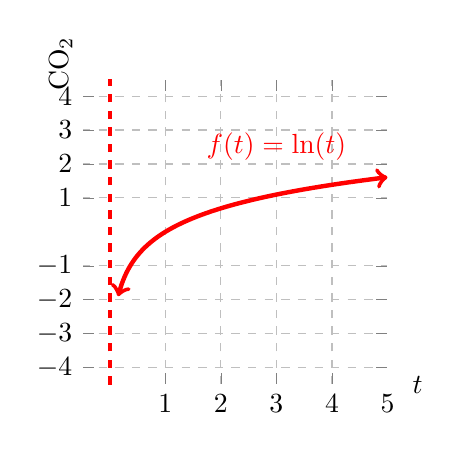
\begin{tikzpicture}[scale=1]
          \begin{axis}[
       %     axis y line = none,
        %   axis x line = bottom,
        	    y axis line style={white},
        	    ylabel={CO$_2$},
            xlabel={$t$},
            x label style={  at={(ticklabel* cs:1.05)},  anchor=west,},
            xtick       = {1,2,3,4,5},
            xticklabels = {$1$,$2$,$3$,$4$,$5$},
            ytick       = {-4,-3,-2,-1,1,2,3,4},
            yticklabels = {$-4$,$-3$,$-2$,$-1$,$1$,$2$,$3$,$4$},
            y label style={  at={(ticklabel* cs:1.05)},  anchor=south,},
            samples     = 160,
            domain      = 0:5,
            restrict y to domain=-4:4,
            xmin = -.5, xmax = 5,
            ymin = -4.5, ymax = 4.5,
            grid=both, grid style=dashed,
            width=2.15in, height=2.15in
          ]
          % pieces 1 and 2
          \addplot[domain=.15:5, red, ultra thick, <->] {ln(x))};
          \node[text=red] at (3,2.5) {$f(t)=\ln(t)$};
           \draw[ultra thick, red, dashed, -] (0,-4.5) -- (0,4.5);
        \end{axis}
    \end{tikzpicture}
    \captionof*{figure}{\blue{Graph of typical\\ logarithmic function: \\$f(t)=\ln(t)$}}
    \end{center}
}{
  \begin{center}
     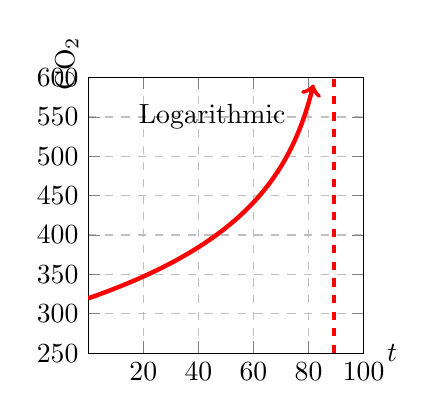
\begin{tikzpicture}[scale=1]
          \begin{axis}[
        %    axis y line = left,
        %    axis x line = bottom,
        	    ylabel={CO$_2$},
            xlabel={$t$},
            x label style={  at={(ticklabel* cs:1.05)},  anchor=west,},
            xtick       = {20,40,60,80,100},
            xticklabels = {$20$,$40$,$60$,$80$,$100$},
            ytick       = {250,300,350,400,450,500,550,600},
            yticklabels = {$250$,$300$,$350$,$400$,$450$,$500$,$550$,$600$},
            y label style={  at={(ticklabel* cs:1.05)},  anchor=south,},
            samples     = 160,
            domain      = 0:100,
            restrict y to domain=250:600,
            xmin = 0, xmax = 100,
            ymin = 250, ymax = 600,
            grid=both, grid style=dashed,
            width=2in, height=2in
          ]
          % pieces 1 and 2
          \addplot[domain=0:100, red, ultra thick, ->] {-109.128*ln(-.0006*x+.0535)};
          \node at (45,550) {\red{Logarithmic}};
            \draw[ultra thick, red, dashed, -] (89.17,250) -- (89.17,600);
           % \addplot[domain=0:60, blue, ultra thick, ->] {1.5 *x +316};
         % \node at (1,4) {$e^t$};
        \end{axis}
    \end{tikzpicture}
     \captionof*{figure}{\blue{Graph of  logarithmic trend line of Keeling Data and asymptote at $x=89.17$}}
    \end{center}
}{
  \begin{center}
     \begin{tikzpicture}[scale=1]
          \begin{axis}[
        %    axis y line = left,
        %    axis x line = bottom,
        	    ylabel={CO$_2$},
            xlabel={$t$},
            x label style={  at={(ticklabel* cs:1.05)},  anchor=west,},
            xtick       = {20,40,60,80,100},
            xticklabels = {$20$,$40$,$60$,$80$,$100$},
            ytick       = {250,300,350,400,450,500,550,600},
            yticklabels = {$250$,$300$,$350$,$400$,$450$,$500$,$550$,$600$},
            y label style={  at={(ticklabel* cs:1.05)},  anchor=south,},
            samples     = 160,
            domain      = 0:100,
            restrict y to domain=250:600,
            xmin = 0, xmax = 100,
            ymin = 250, ymax = 600,
            grid=both, grid style=dashed,
            width=2in, height=2in
          ]
          % pieces 1 and 2
          \begin{pgfonlayer}{background}
           	\fill [lightgray] (89.17,250) rectangle (100,600);
	\end{pgfonlayer}
	\node at (40,275) {\red{Log undefined}};
	\draw[ thick, red, ->] (75,275) -- (95,275);
                       \addplot[domain=0:100, blue, ultra thick, ->] {76.8748*e^(.0142*x)+242.763};
%	\node at (40,275) [label={[align=left] Logarithm\\undefined}]{};
          \addplot[domain=0:100, red, ultra thick, ->] {-109.128*ln(-.0006*x+.0535)};
              \node at (45,550) {\red{Logarithmic}};
            \draw[ultra thick, red, dashed, -] (89.17,250) -- (89.17,600);
                       \addplot[domain=0:100, blue, ultra thick, ->] {76.8748*e^(.0142*x)+242.763};
             \node at (70,350) {Exponential};
           % \addplot[domain=0:60, blue, ultra thick, ->] {1.5 *x +316};
         % \node at (1,4) {$e^t$};
        \end{axis}
    \end{tikzpicture}
     \captionof*{figure}{\blue{Graph of logarithmic and exponential trend lines. Logarithm is undefined in gray region. }}
    \end{center}
}
{\em Summary!} 
\itemI{
\item  Linear function from trend line {\em does not} reflect scientists belief.
\item Exponential function from trend line {\em does} reflect scientists belief.
\item Logarithmic function from trend line {\em does} reflect scientists belief on $0\ds \leq t < \frac{535}{6}$. 
\item Logarithmic function from trend line is undefined  for $\ds t \geq \frac{535}{6}$  and {\em ceases to become a working model}.
}
    }
 \newpage
\item   Which best-fit function based on the data set from Screen 1 in Desmos would you recommend to policy makers to predict how fast CO2 in the atmosphere will change in the future?  Articulate at least two reasons why you made your recommendation and at least 1 possible weakness of your recommendation. Note that a more complete data set from 1960 to 2025 is available on Screen 2 of Desmos and might be helpful to test/refine your recommendation. \label{qNum2}

\sol{
There is more than one reasonable answer to this question. Here is one:\\
\\
We recommend the exponential model because
\itemI{
\item It best reflects the belief that not only is the amount of CO$_2$ in the atmosphere growing, but that the growth rate is speeding up.
\item Using data from the 2nd screen we see that in 2025, i.e. $t=60$, there are $426$ ppm of CO$_2$ in the atmosphere. When we compare predictions from all of our models we see that the exponential model does the best job (although the quadratic model is not far behind).
\itemC{
\item $\ds c_{exponential}(60)=424.0675$ ppm
\item $\ds c_{linear}(60)=408.196$
\item $\ds c_{quadratic}(60)=421.512$ 
\item  $\ds c_{log}(60)=441.4833$.
}
\item  $R^2=0.9994$ for the exponential model is only very slightly better than other models. This is not as strong a reason as some other rationales.
}

{\em Some weakness of the exponential model} 
\itemI{
\item It will continue to grow forever towards infinity. At some point, this model ceases to be realistic.
\item We are using a small subset of data to create our lines of best fit to predict what happens in 2025 when more data since 2010 is available.
}
}
 \vs{.25}
\item Click ``Next" in upper right corner to go to Screen 2 in Desmos.  This screen  contains a more complete data set from 1960 to 2025.   {\em Use the function you recommended to policy makers in \#\ref{qNum2}} to calculate the average rate of change (up to $2$ decimal places) from 2000 to 2025.  What does this value suggest about future change in the amount of atmospheric CO$_2$? See {\em Creating Functions and Functions of Best Fit} at the end of this document for instructions on how to create functions in Desmos.
\sol{ 
Your answer will only need to utilize their recommended function. However answers for all follow.\\\\
The year 2000 occurs at $t=35$ and the year 2025 occurs at $t=60$.  
\itemI{
\item Linear function:  Average Rate of Change: $\ds \frac{c_{linear}(60)-c_{linear}(35)}{60-35}\approx 1.53$ ppm per year (from Desmos). \\
This means that the change per year for  $\ds 35\leq t\leq 60$ is, on average, $1.53$ ppm per year.
\item Quadratic function:  Average Rate of Change: $\ds \frac{c_{quadratic}(60)-c_{quadratic}(35)}{59-35}\approx 2.08$ ppm per year (from Desmos). \\
This means that the change per year for  $\ds 35\leq t\leq 60$ is, on average, $2.08$ ppm per year.
\item Exponential function:  Average Rate of Change: $\ds \frac{c_{exponential}(60)-c_{exponential}(35)}{60-35}\approx 2.18$ ppm per year (from Desmos). \\
This means that the change per year for  $\ds 35\leq t\leq 60$ is, on average, $2.18$ ppm per year.
\item Logarithmic function:  Average Rate of Change: $\ds \frac{c_{log}(60)-c_{log}(35)}{60-35}\approx 2.70$ ppm per year (from Desmos). \\
This means that the change per year for  $\ds 35\leq t\leq 60$ is, on average, $2.70$ ppm per year.
}

}
\newpage
 \item A ``tipping point" is the amount of CO$_2$ in the atmosphere after which, the growth rate begins to accelerate.  Mendez and Farazmand (2021)\footnote{Mendez, A., \& Farazmand, M. (2021). Investigating climate tipping points under various emission reduction and carbon capture scenarios with a stochastic climate model. Proceedings of the Royal Society A: Mathematical, Physical and Engineering Sciences, 477(2256). https://doi.org/10.1098/rspa.2021.0697} claim this will occur when there is $478$ ppm of CO$_2$ in the atmosphere. 
 \enum{
 \item In what year does your recommended model predict we will reach a tipping point?  Clearly explain how you arrived at your answer. 
 \sol{
 If you chose any recommended model besides a linear function, you will likely will not have the tools to algebraically solve for the correct time.  Thus, use of technology is highly encouraged here! 
 
 In Desmos, if your recommended trend line function and $c(t)=478$ are both graphed, a grey point is placed at point of intersection. Hover over this point to see details.\\
 
 
 You are only required to use your recommended function to answer this question. However we are providing solutions for all possible trendline functions.  We're labeling the answer as ``$t^*$" for the purpose of utilizing this same value in next question.
 \itemI{
  \item Linear:  $t^*=105.39$ (hovering over intersection of graph of $y=478$ and $c_{linear}(t)$ in Desmos).  This corresponds to  mid-May of 2070.
 \item Quadratic:  $t^*=81.84$ (hovering over intersection of graph of $y=478$ and $c_{quadratic}(t)$ in Desmos).  This corresponds to early November of 2046.
 \item Exponential:   $t^*=78.21$ (hovering over intersection of graph of $y=478$ and $c_{exponential}(t)$ in Desmos).  This corresponds to mid-March of 2043.
  \item Logarithmic:   $t^*=68.29$ (hovering over intersection of graph of $y=478$ and $c_{log}(t)$ in Desmos).  This corresponds to mid-April of 2033.
 }
 }
 %vs{.1}
 \item {\em Estimate} the growth rate (to two decimal places) when the tipping point is reached.   Describe how you made your estimate and don't forget use appropriate units!. 
 \nti{
Students have the tools to calculate the instantaneous growth rate for the linear and quadratic models since we have not talked about the Chain Rule nor how to take derivatives of logarithmic functions. Thus, they are only required to estimate this quantity.  A liberal use of technology is suggested here.  
\itemI{
\item Students will need to choose 2 points relatively close together and calculate Average Rate of Change
\item We haven't talked about how to characterize ``relatively close", so we will probably want to grade student work by asking ``is this a {\em reasonable} estimate?"
\item Many students will know how to set up a slider in Desmos, which will make quick work of generating many estimates of $\ds \frac{f(t^*+h)-f(t^*)}{h}$
\item We also have not talked about how to ensure that we are within $2$ decimal places of actual answer.  
}
Suggested prompts:
\itemI{
\item How have we talked about estimating instantaneous growth rates in class?
\item Think about how we calculated Average Rate of Change earlier in class. Can we adopt that approach here?  
\item How close to year $t^*$ should you get to ensure you will be accurate to within $2$ decimal places? What if you keep getting closer and closer and the final answer ceases changing in first $2$ decimal places?
}

Only one estimate is required for this question. 
 \itemI{
  \item Linear:  Slope of $\ds c_{linear}(t)=1.5321\,t+316.527$ is $1.5321$. To two decimal places, IROC is $1.53$ ppm of CO$_2$ per year.  \\
  Interpretation:  when  $t^*=105.39$,  CO$_2$ is increasing by $1.53$ ppm per year.
 \item Quadratic:  $t^*=81.84$ (from part a)). 
 \itemI{
 \item $\ds \frac{c_{quadratic}(t^*+h)-c_{quadratic}(t^*)}{h}=2.84$ when $h=1$
 \item $\ds \frac{c_{quadratic}(t^*+h)-c_{quadratic}(t^*)}{h}=2.83$ when $h=0.014$ or less and last two decimal  places appear to not change for smaller $h$.
 }
  Interpretation:  when  $t^*=81.84$,  CO$_2$ is increasing by $2.83$ ppm per year.\\
  (Exact answer happens to be $\ds c_{quadratic}^{\prime}(81.81)=2.825312\dots$)
 \item Exponential:   $t^*=78.76$ (from part a)). 
 \itemI{
\item $\ds \frac{c_{exponential}(t^*+h)-c_{exponential}(t^*)}{h}=3.39$ when $h=1$
 \item $\ds \frac{c_{exponential}(t^*+h)-c_{exponential}(t^*)}{h}=3.36$ when $h=0.047$  or less and last two decimal  places appear to not change for smaller $h$.
 }
  Interpretation:  when  $t^*=78.21$,  CO$_2$ is increasing by $3.39$ ppm per year.\\
  (Exact answer happens to be $\ds c_{exponential}^{\prime}(78.21)=3.3638\dots$)
  \item Logarithmic:   $t^*=68.29$ (from part a)).  
  \itemI{
\item $\ds \frac{c_{log}(t^*+h)-c_{log}(t^*)}{h}=5.36$ when $h=1$
\item $\ds \frac{c_{log}(t^*+h)-c_{log}(t^*)}{h}=5.23$ when $h=.0616$ or less and last two decimal  places appear to not change for smaller $h$.
}
  Interpretation:  when  $t^*=68.29$,  CO$_2$ is increasing by $3.34$ ppm per year.\\
  (Exact answer happens to be $\ds c_{log}^{\prime}(68.29)=5.2272\dots$)
 }
 }
}


}

  \newpage
%%%%% Instructions used in both pre-class and during-class portion %%%%%%

      \begin{center}{\bf Creating Functions  and Functions of Best Fit}\end{center}
  \vs{.1}
  {\large \em Using Desmos/Amplify for this Application}
  \itemC{
  \item Go to \href{https://student.amplify.com/}{\underline{student.amplify.com}} or \href{https://student.desmos.com/}{\underline{student.desmos.com}}.  
  \item You will need to  use code \desmosClassCode.
  \item You might need to register for an Amplify  account (it's free).  If so, please use your UVA email as this helps us keep track of what work your group does.
  }~\\
  {\large \em Creating Functions of Best Fit in Desmos/Amplify} \hs{.1} Functions of best fit are sometimes referred to as trend lines, regression functions or least squares lines of best fit.  The following steps will explain how to use Desmos to create functions of best fit and to find the R$^2$-value for a given set of data.
\enum{
\item {\em (This step has already been done for you.)} Go to desmos.com/calculator and create a table of data. Cut-paste from a spreadsheet is probably the most straightforward way to generate this table.  Other options are here: \red{\underline{\url{https://help.desmos.com/hc/en-us/articles/4405489674381-Tables}}} \vs{-.15}
\item {\em (This step has already been done for you.)} Find the default header for a table generated by cut-paste. It likely will be $(x_1, y_1)$. Change it to whatever you like. For example, $(t_1,c_1)$.
\item In another cell, create the linear function of best fit using variables from the header. For example
$$c_1 \sim mt_1+b$$ will create a linear best-fit function. Values for $R^2$ and   parameters $m$ and $b$ will be generated.\\
}
{\bf The following steps are not needed for pre-class activity but will be used during class.}
\enum{ \setItemnumber{4}
\item A quadratic function of best fit can be created by $\ds c_1 \sim at_1^2+bt_1+c$.  Values for $R^2$ and parameters $a$, $b$, and $c$ will be generated.
\item An exponential function of best fit can be created by  $\ds c_1 \sim a e^{b\, t_1} +c$.  Values for $R^2$ and parameters $a$, $b$, and $c$ will be generated.
\item A logarithmic function of best fit can be created by $\ds c_1 \sim a \ln(b\, t_1 +c)$. Values for $R^2$ and all parameters $a$, $b$, and $c$ will be generated.
}

    {\large \em Creating and Graphing Functions in Desmos/Amplify}
   \itemI{
   \item  Create expression cell by clicking on {\Large$+$} in the upper left corner.  Choose ``{\em $f(x)$ expression}".
   \item Type the function definition in any empty cell in left column of Desmos. For example,\\ $f(t)=3t+6$. Graphs will automatically be created while defining the function. 
   \item Function names in Desmos will utilize a single letter for the dependent variable For example, $f(t)$, $g(t)$, $h(t)$ are all acceptable function names. $Lin(t)$ or $Exp(t)$ will not be accepted by Desmos. 
   \item Subscript notation {\em can} be used in naming conventions. For example $f_{linear}(t)$ and $f_{exponential}(t)$  name two different functions.
   \item To evaluate functions at a specific value, say $t=10$,  use an empty expression cell to type in $f(1)$. The result is automatically displayed.
   }
{\large \em Data sets used in Desmos} \hs{.1}  Feel free to use these data sets in whatever tool is helpful.
\itemC{
  \item 1965 to 2010 data: \\ \red{\underline{\url{https://docs.google.com/spreadsheets/d/1KvLYR1DRHiRrkb1dh-qrSMRwzKPKuH1SkMDghl2fTcc/}}}
  \vs{-.1}
  \item 1960 to 2025 data:\\ \red{\underline{ \url{https://docs.google.com/spreadsheets/d/1dtNawrPd3W744p229R7WS83KKHVkyEokcsyCeyPDF4w}}}
  }



\end{document}  